
\newpage
\section{Model-Specific Post-hoc Methods}\label{sec:5}

Model-specific post-hoc methods are limited to a specific type of model. In the following section, we examine the vanilla gradient method, which is only suitable for models that allow gradient computation. For instance, this method is not feasible for Decision Trees due to their inherent structure.

\subsection*{Image-Specific Class Saliency (Vanilla Gradient Method)}

\begin{table}[H]
  \centering
  \begin{tabular}{|p{0.17\textwidth}|p{0.77\textwidth}|}
    \hline
    Form of \newline explanation & 
    Feature visualization. \\
    
    \hline
    Interpretation & 
    Pixels that strongly influence the prediction of the neural network are identified. \\
    \hline
    Advantages &
    \begin{itemize}[nosep, left=0em]
        \item easy to immediately recognize the important regions of the image to the model's prediction
    \end{itemize} \\
    
    \hline
    Disadvantages &
    \begin{itemize}[nosep, left=0em]
        \item tells only where the network is looking not why the prediction was made
        \item can be highly unreliable
    \end{itemize} \\
    
    \hline
    Properties & 
    post-hoc, model-specific, local  \\
    
    \hline
  \end{tabular}
  \caption[Overview XAI - Image-Specific Class Saliency (Vanilla Gradient method)]{Overview XAI - Image-Specific Class Saliency (Vanilla Gradient method).}
  \label{tab:VanillaGradient}
\end{table}

The Vanilla Gradient method, also known as "Image-Specific Class Saliency" by its authors, falls within the category of gradient-based pixel attribution techniques. Saliency maps generated by these methods highlight the pixels considered significant by a neural network during the process of image classification.\\
The computation of a saliency map using the Vanilla Gradient method is relatively straightforward. Instead of calculating the gradient of the output regarding the network's weights, as done in typical backpropagation, the gradient of the output regarding the input image is computed: $\frac{\delta f(I;W)}{\delta I}$. Therefore, each pixel in the image has a corresponding gradient value, which can afterward be used for visualization. Pixels with higher absolute gradient values are considered more important in influencing the network's decision. An example of the Vanilla gradient method is shown in the following figure:

\begin{figure}[H]
    \centering
    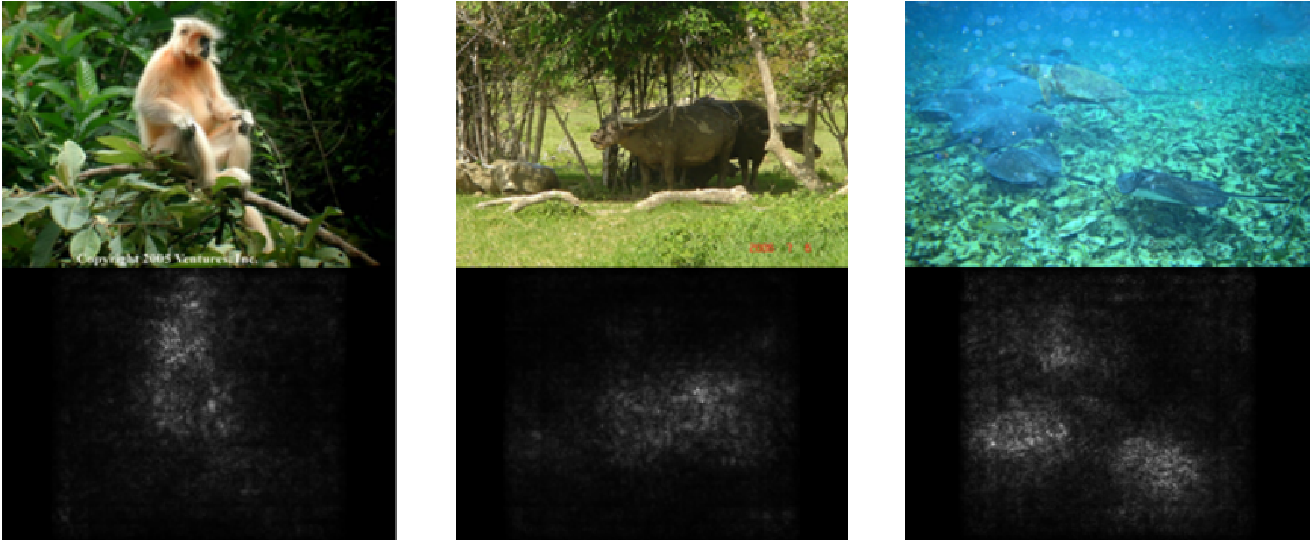
\includegraphics[width=0.9\linewidth]{pics/sal_map.pdf}
    \caption[Image-specific class saliency maps.]{Image-specific class saliency maps for the top-1 predicted class in ILSVRC-2013 test images. The maps were extracted using a single back-propagation pass through a classification ConvNet.\cite{simonyan2014deep}}
    \label{fig:sal_ap}
\end{figure}
As you can see the interpretation is easy and by performing only one backpropagation step the computation is fast and efficient. 

However, what meaningful conclusions can one derive from the highlighted pixels? \cite{Ghorbani_Abid_Zou_2019} demonstrates that minor perturbations to the input image result in nearly identical saliency maps, yet the neural network may classify the output differently. For instance, as illustrated in Figure \ref{fig:saliency_husky}, an image of a husky was misclassified as a flute, despite having very similar saliency maps.

\begin{figure}[H]
    \centering
    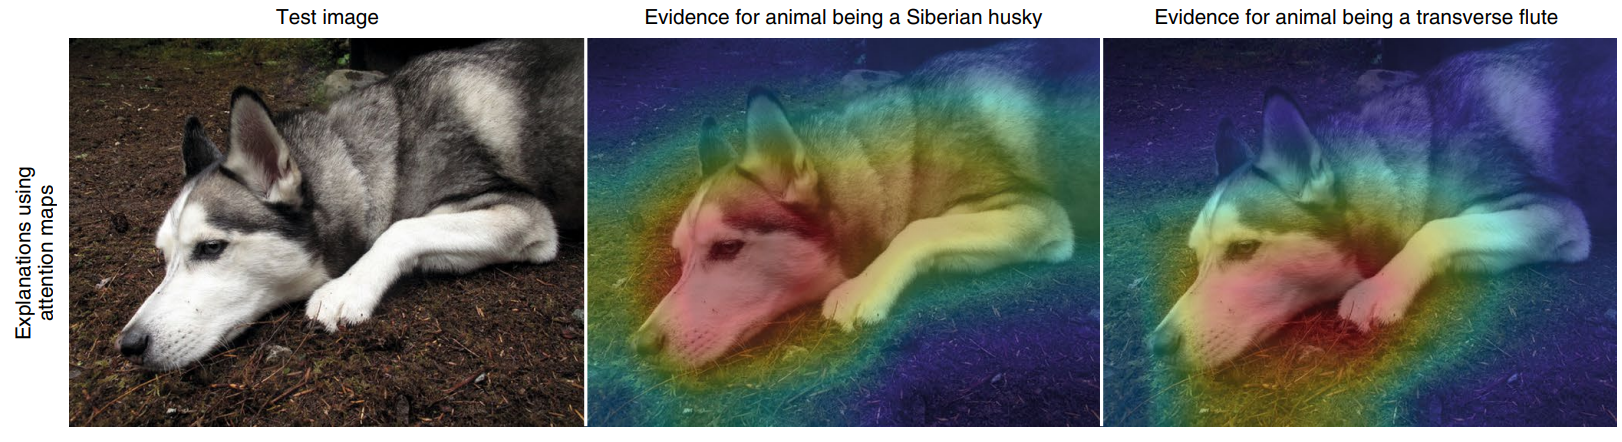
\includegraphics[width=0.9\linewidth]{pics/saliency_husky.png}
    \caption[Image is labeled as a dog and a musical instrument when the saliency maps look essentially the same.]{Image is labeled as a dog and a musical instrument when the saliency maps look essentially the same. \cite{Ghorbani_Abid_Zou_2019}}
    \label{fig:saliency_husky}
\end{figure}

So while the saliency map provides insight into the regions of focus within a neural network, it fails to explain the reason behind the network's specific prediction\cite{rudin2019stop}.

\cite{Ghorbani_Abid_Zou_2019} also demonstrated that saliency maps display considerable unreliability. Even minor perturbations to an image can lead to substantial changes in the saliency map, despite the network's prediction remaining the same. The example shown in Figure \ref{fig:advers} illustrates this phenomenon using three images:

\begin{figure}[H]
    \centering
    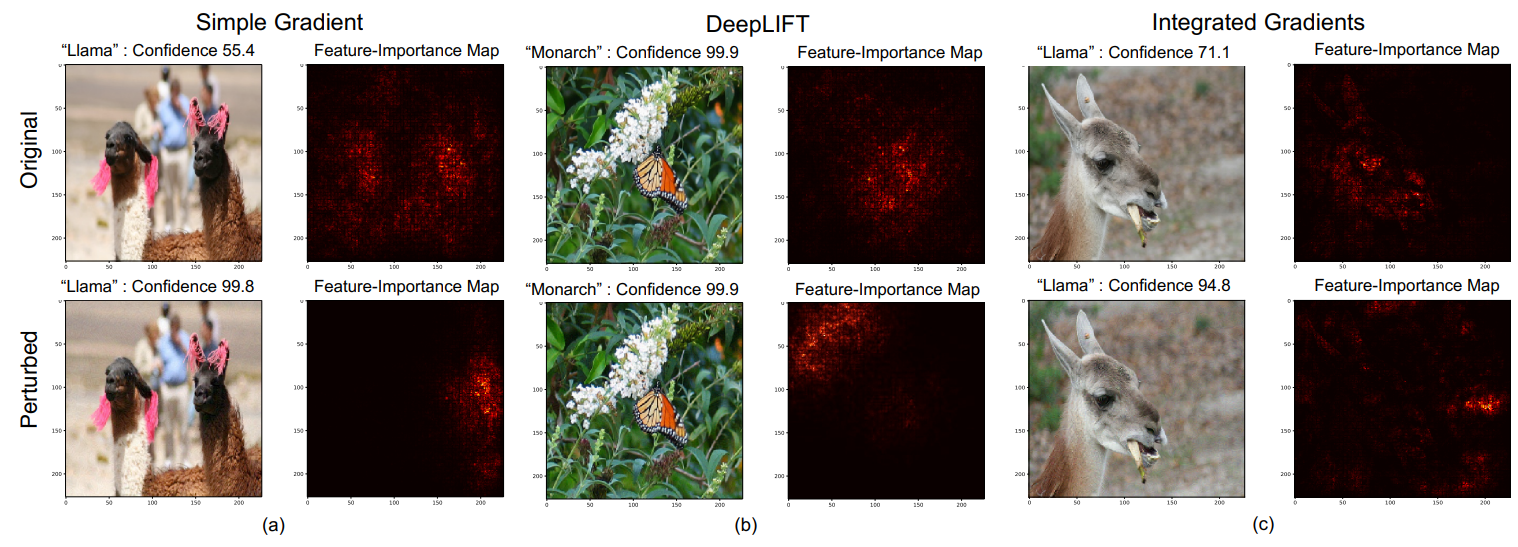
\includegraphics[width=0.9\linewidth]{pics/advers.png}
    \caption[Adversarial attack against feature-importance maps.]{Adversarial attack against feature-importance maps. The top row shows the the original images and their saliency maps and the bottom row shows the perturbed images and the corresponding saliency maps.\cite{Ghorbani_Abid_Zou_2019}}
    \label{fig:advers}
\end{figure}

In each of the three images, the predicted classification remains the same despite the introduced perturbation. However, the saliency maps of the perturbed images have a notable shift towards pixels that typically wouldn't be considered as influential according to human perception.
